\documentclass[aspectratio=169]{beamer}
\usepackage{graphicx}
\usepackage{listings}
\lstset{
    basicstyle=\ttfamily
}

\usepackage{hyperref}

\usetheme{metropolis}
\title{Understanding why Projects Fail}
\institute{Engineers for Exploration, UC San Diego}
\logo{
\includegraphics[height=0.62cm,keepaspectratio]{e4e_logo_350x136.png}}
\setbeamertemplate{caption}[numbered]

\begin{document}
\maketitle
\begin{frame}
    We know projects fail.  Why?
\end{frame}
\begin{frame}
    When are good times to figure out why projects fail?
    \centering
    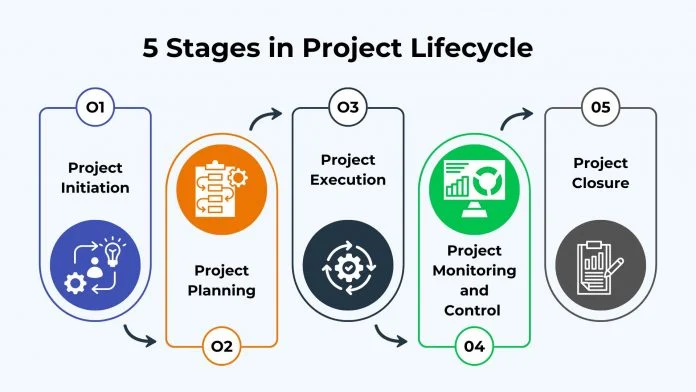
\includegraphics[width=.8\textwidth,height=0.7\textheight,keepaspectratio]{17_project_lifecycle.png}
\end{frame}
\begin{frame}
    Introducing:
    \begin{itemize}
        \item Pre-mortems
        \item Post-mortems
    \end{itemize}
\end{frame}
\section{Post-mortem}
\begin{frame}{What is a Post-mortem?}
    \begin{itemize}[<+->]
        \item Learning from past experiences
        \item Increasing team communication
        \item Improving team morale
    \end{itemize}
\end{frame}
\begin{frame}{6 R's of Effective Debriefs}
    \begin{itemize}[<+->]
        \item Reflection
        \item Reconvene
        \item Reset
        \item Review
        \item Refine
        \item Recap
    \end{itemize}
\end{frame}
\begin{frame}{Reflection}
    Allows the team to:
    \begin{itemize}
        \item Return from any emotional highs or lows
        \item Individually identify concerns/feedback
    \end{itemize}
\end{frame}
\begin{frame}{Reconvene}
    \begin{itemize}
        \item Set a time
        \item When is too late?
        \item When is too early?
        \item When to decide the time?
    \end{itemize}
\end{frame}
\begin{frame}{Reset}
    \begin{itemize}
        \item No ego, no rank
        \item Reduce authority gradient
        \item Only one role - facilitator
    \end{itemize}
\end{frame}
\begin{frame}{Review}
    \begin{itemize}
        \item Identify objectives/goals
        \item Assess performance
        \item Use context rich stories
        \item Provide feedback
    \end{itemize}
\end{frame}
\begin{frame}{Refine}
    \begin{itemize}
        \item Plan for getting/doing better
        \item Focus on individual and team performance
    \end{itemize}
\end{frame}
\begin{frame}{Recap}
    \begin{itemize}
        \item Review all learnings
        \item Make sure everyone is on the same page
    \end{itemize}
\end{frame}
\section{Pre-mortem}
\begin{frame}{What is a Pre-mortem?}
    \begin{itemize}[<+->]
        \item Apply learning from past experiences - prospective hindsight
        \item Increasing team communication - align on project risks, involve cross-functional teams
        \item Proactive risk assessment - reduce overconfidence
    \end{itemize}
\end{frame}
\begin{frame}{Steps to conducting a pre-mortem}
    \begin{itemize}[<+->]
        \item Create a plan
        \item Identify potential project failures
        \item Share risks
        \item Identify risks with high likelihood and/or severity
        \item Review and revise project plan
    \end{itemize}
\end{frame}
\end{document}